\documentclass[10pt,twocolumn,letterpaper]{article}
\usepackage[utf8]{inputenc}
\usepackage[T1]{fontenc}
\usepackage{mathptmx}
\usepackage[margin=0.75in,columnsep=0.25in]{geometry}
\usepackage{amsmath}
\usepackage{graphicx}
\usepackage{booktabs}
\usepackage{tabularx}
\usepackage{array}
\usepackage[font=footnotesize,labelsep=colon]{caption}
\usepackage{titlesec}
\usepackage{enumitem}
\usepackage{xcolor}
\usepackage[hidelinks]{hyperref}

% Nombres en español (sin babel-spanish)
\renewcommand{\figurename}{Fig.}
\renewcommand{\tablename}{TABLA}
\renewcommand{\refname}{Referencias}
\renewcommand{\abstractname}{Resumen}
\renewcommand{\thetable}{\Roman{table}}

% Estilo de secciones tipo IEEE
\renewcommand{\thesection}{\Roman{section}}
\renewcommand{\thesubsection}{\Alph{subsection}}
\titleformat{\section}{\centering\normalsize\scshape}{\thesection.}{0.5em}{}
\titleformat{\subsection}{\normalsize\itshape}{\thesubsection.}{0.5em}{}
\titlespacing*{\section}{0pt}{1.2ex}{0.8ex}
\titlespacing*{\subsection}{0pt}{1ex}{0.5ex}
\setlist{nosep,leftmargin=1.2em}

\newcommand{\fig}[3]{%
\begin{figure}[!htbp]\centering
\includegraphics[width=#3\columnwidth]{img/#1}
\caption{#2}\label{fig:#1}
\end{figure}}

\begin{document}

\twocolumn[{%
\begin{center}
{\LARGE Diseño e Implementación de un Amplificador de\\[2pt] Potencia Multietapa Clase AB\par}
\vspace{1em}
{\large Felipe Aviles Castro, Brahiam Alberto Campiño Romero\par}
\vspace{0.3em}
{\itshape Universidad de Ibagué\par}
{\small brahiam.campino@estudiantesunibague.edu.co\par}
\vspace{1.2em}
\end{center}}]

\noindent\textbf{\textit{Resumen}---En el presente trabajo se desarrolló el diseño e implementación de un amplificador de potencia multietapa orientado a amplificar la señal de audio de un teléfono celular hasta niveles de potencia adecuados para un parlante de \(8\,\Omega\). El sistema está compuesto por cuatro etapas: una etapa JFET en autopolarización, una etapa en emisor común (EC), una etapa colector común (CC) en configuración Darlington y una etapa de potencia push-pull clase AB. El diseño requirió múltiples iteraciones de cálculo y ajuste debido a problemas de adaptación de impedancias, estabilidad térmica y limitaciones prácticas de montaje. El amplificador fue diseñado para una entrada de 200~mVp y una salida de aproximadamente 10~Vp y 1.25~Ap sobre la carga, lo que corresponde a una potencia promedio de diseño de \(\approx 6.25\)~W para señal senoidal. En las pruebas experimentales se observaron picos de salida de hasta 11.1~V, equivalentes a una potencia instantánea pico de \(\approx 15\)~W y a una potencia promedio estimada entre 5 y 8~W. Las observaciones prácticas fueron coherentes con los cálculos teóricos.}

\vspace{0.5em}
\noindent\textbf{\textit{Palabras clave}---Amplificador clase AB, JFET, Darlington, colector común, emisor común, adaptación de impedancias.}

\section{Introducción}
Los amplificadores de potencia son dispositivos fundamentales en sistemas electrónicos debido a su capacidad de entregar energía suficiente a cargas de baja impedancia manteniendo la integridad de la señal. Sin embargo, su diseño implica desafíos relacionados con la estabilidad térmica, la transferencia de potencia y la adaptación de impedancias entre etapas.

En este proyecto se desarrolló un amplificador de potencia multietapa compuesto por un JFET, una etapa en emisor común, una etapa buffer en colector común Darlington y una etapa de salida clase AB, con el propósito de amplificar la señal de audio de un celular hacia un parlante buscando la mayor potencia posible. El objetivo principal fue obtener una ganancia total de voltaje aproximada de
\begin{equation}
A_v = 50
\end{equation}
a partir de una señal de entrada de
\begin{equation}
V_{in} = 200\ \text{mVp}
\end{equation}
garantizando además una adecuada entrega de corriente hacia la carga.

\section{Especificaciones del diseño}
Los parámetros iniciales del diseño se resumen en la Tabla~\ref{tab:param}. La potencia en la carga se expresa en vatios (W), ya que la carga es resistiva; para una señal senoidal de amplitud \(V_p\) sobre una carga \(R_L\):
\begin{equation}
P_{pico} = \frac{V_p^2}{R_L}, \qquad P_{prom} = \frac{V_p^2}{2R_L} = \frac{V_p I_p}{2}.
\end{equation}

\begin{table}[!h]\centering
\caption{Parámetros iniciales}\label{tab:param}
\begin{tabular}{@{}ll@{}}
\toprule
Parámetro & Valor\\
\midrule
Voltaje de entrada & 200 mVp\\
Voltaje de salida requerido & 10 Vp\\
Carga & \(8\,\Omega\)\\
Corriente pico requerida & 1.25 Ap\\
Potencia pico instantánea & 12.5 W\\
Potencia promedio (senoidal) & 6.25 W\\
Alimentación & 25 V\\
Ganancia total de voltaje & \(A_v = 50\)\\
Ganancia total de corriente\(^{*}\) & \(A_i = 6.25\times10^{6}\)\\
\bottomrule
\multicolumn{2}{@{}p{0.9\columnwidth}@{}}{\footnotesize \(^{*}\)Calculada como \(I_{p,carga}/I_{p,in}\) con \(I_{p,in} = 200\ \text{mV}/1\ \text{M}\Omega = 200\ \text{nA}\), es decir, suponiendo una resistencia de entrada de \(1\ \text{M}\Omega\) en la etapa JFET.}
\end{tabular}
\end{table}

\begin{table}[!h]\centering
\caption{Dispositivos utilizados}\label{tab:disp}
\begin{tabular}{@{}ll@{}}
\toprule
Etapa & Dispositivo\\
\midrule
JFET autopolarizado & 2SK30 (canal N)\\
Emisor común & 2N3904\\
Colector común Darlington & 2 transistores TIP\(^{\dagger}\)\\
Amplificador clase AB & TIP31C y TIP32C\\
\bottomrule
\multicolumn{2}{@{}p{0.9\columnwidth}@{}}{\footnotesize \(^{\dagger}\)Ver la Sección~\ref{sec:erratas}, punto~2.}
\end{tabular}
\end{table}

\section{Desarrollo del diseño}
\subsection{Etapa de potencia clase AB}
El diseño inició a partir de la etapa de potencia clase AB debido a que esta determina las condiciones de carga necesarias para las etapas anteriores. Inicialmente se realizaron modificaciones al circuito visto en laboratorio, agregando resistencias de potencia en la salida con el fin de reducir la distorsión y mejorar la estabilidad frente a variaciones de señal.

Posteriormente se observó que la resistencia de entrada calculada era demasiado baja, afectando negativamente la adaptación de impedancias. Debido a esto se aumentó el voltaje de polarización y se modificó el valor de la resistencia \(R_2\), permitiendo incrementar la resistencia de entrada de la etapa.

La etapa clase AB se implementó con un par complementario TIP31C (NPN, \(\beta \approx 140\)) y TIP32C (PNP, \(\beta \approx 154\)), con un beta promedio de
\begin{equation}
\beta \approx 147
\end{equation}
y una alimentación de \(V_{CC} = 25\) V, que cumple el criterio \(V_{CC} > 2V_L\). Además, a la salida del Darlington se añadió una resistencia de potencia debido a la elevada corriente que circula en esta región del circuito. Los cálculos se muestran en las Figs.~\ref{fig:fig01_calc_ab_1} y~\ref{fig:fig02_calc_ab_2}.

\fig{fig01_calc_ab_1}{Cálculos de la etapa clase AB: corriente de carga, criterio de alimentación y análisis DC.}{0.7}
\fig{fig02_calc_ab_2}{Cálculos de la etapa clase AB: modelo AC y dimensionamiento de \(R_2\).}{0.7}

\subsection{Etapa JFET en autopolarización}
La primera etapa de amplificación fue implementada mediante un transistor JFET 2SK30 de canal N en configuración de autopolarización. Esta etapa fue seleccionada debido a su alta impedancia de entrada y su capacidad para amplificar señales pequeñas sin cargar significativamente la fuente. A partir de los parámetros medidos del dispositivo (\(V_P \approx -2.44\) V, \(I_{DSS} \approx 2.3\) mA) y de la ecuación de Shockley se obtuvo el punto de operación \(V_{GS} \approx -0.93\) V, \(I_D \approx 1.06\) mA, con una transconductancia \(g_m \approx 1.42\) mS (Fig.~\ref{fig:fig03_calc_jfet_1}).

La etapa fue diseñada para proporcionar una ganancia aproximada de
\begin{equation}
A_{v(JFET)} \approx 5
\end{equation}
cargada con la resistencia de entrada de la etapa EC (\(\approx 16\) k\(\Omega\)), lo que llevó a una resistencia de drenador de \(R_D \approx 15.9\) k\(\Omega\) (Fig.~\ref{fig:fig04_calc_jfet_2}). Durante el diseño se encontró que la resistencia de carga debía mantenerse relativamente baja para evitar un aumento excesivo de la resistencia reflejada hacia las etapas siguientes.

\fig{fig03_calc_jfet_1}{Cálculos de polarización y transconductancia de la etapa JFET.}{0.7}
\fig{fig04_calc_jfet_2}{Cálculos de ganancia de la etapa JFET y ganancias globales del sistema.}{0.7}

\subsection{Etapa emisor común}
La segunda etapa consistió en un transistor 2N3904 en configuración emisor común, diseñada para proporcionar una ganancia aproximada de
\begin{equation}
A_{v(EC)} \approx 10
\end{equation}
con un beta aproximado de
\begin{equation}
\beta = 300.
\end{equation}
La resistencia de emisor se obtuvo a partir de la ganancia requerida y de la resistencia de carga equivalente, que corresponde a la resistencia de entrada de la etapa Darlington (\(\approx 12\) k\(\Omega\)):
\begin{equation}
R_E = 600\ \Omega
\end{equation}
y posteriormente la resistencia reflejada
\begin{equation}
R_{ref} = \beta R_E \approx 180\ \text{k}\Omega.
\end{equation}
Con este valor se calcularon la resistencia de base \(R_B\) y las resistencias del divisor de tensión mediante análisis de mallas y polarización DC. Para garantizar estabilidad térmica se utilizó el criterio
\begin{equation}
R_B = 0.1\,\beta R_E = 18\ \text{k}\Omega
\end{equation}
que aproxima el punto de operación a una condición térmicamente estable. La resistencia de entrada resultante de la etapa fue \(R_{in(EC)} \approx 16.4\) k\(\Omega\), que es la carga vista por la etapa JFET (Figs.~\ref{fig:fig05_calc_ec_1} y~\ref{fig:fig06_calc_ec_2}).

\fig{fig05_calc_ec_1}{Primera iteración de cálculo de la etapa emisor común (con \(V_{CC} = 30\) V, descartada).}{0.7}
\fig{fig06_calc_ec_2}{Cálculo final de la etapa emisor común con \(V_{CC} = 25\) V.}{0.7}

\subsection{Etapa colector común Darlington}
La etapa colector común se implementó con dos transistores en configuración Darlington. La ganancia de corriente del par es aproximadamente el producto de las ganancias individuales, \(\beta_D \approx \beta_1\beta_2\); el valor usado en los cálculos fue
\begin{equation}
\beta_D \approx 18\,000.
\end{equation}
Esta etapa se empleó como buffer de impedancia, debido a que un solo transistor en colector común no proporcionaba suficiente ganancia de corriente ni estabilidad práctica.

Su objetivo es elevar la baja resistencia de entrada de la etapa clase AB hasta un valor que la etapa EC pueda manejar. Como se resume a continuación, en la cadena cada etapa carga a la anterior:
\begin{itemize}
\item La etapa JFET ve como carga \(R_{in(EC)} \approx 16\) k\(\Omega\).
\item La etapa EC ve como carga \(R_{in(D)} \approx 12\) k\(\Omega\), la resistencia de entrada del Darlington.
\item El Darlington ve como carga la entrada de la etapa clase AB.
\end{itemize}
La resistencia de base del Darlington fue calculada a partir de la ecuación de resistencia de entrada \(R_{in} = R_B \parallel h_{fe}(R_E \parallel R_L)\), considerando
\begin{equation}
R_L = R_{in(AB)}.
\end{equation}
En la iteración final (Fig.~\ref{fig:fig08_calc_darlington_2}) se obtuvo \(R_B \approx 12.2\) k\(\Omega\), con valores comerciales \(R_1 = 43\) k\(\Omega\) y \(R_2 = 15\text{--}18\) k\(\Omega\), y una ganancia de corriente de la etapa
\begin{equation}
A_i = \frac{R_{in}}{R_L} \approx 120.
\end{equation}
Posteriormente se verificó que no existieran inconsistencias en las ecuaciones de polarización.

\fig{fig07_calc_darlington_1}{Primera iteración de cálculo de la etapa colector común Darlington (\(A_i \approx 57\)).}{0.7}
\fig{fig08_calc_darlington_2}{Iteración final de la etapa colector común Darlington (\(A_i \approx 120\)).}{0.7}

\subsection{Diseño general en Proteus}
El diseño completo implementado en Proteus se muestra en la Fig.~\ref{fig:fig09_proteus}. Esta simulación permitió verificar el comportamiento general del sistema antes del montaje físico.

\begin{figure*}[!t]\centering
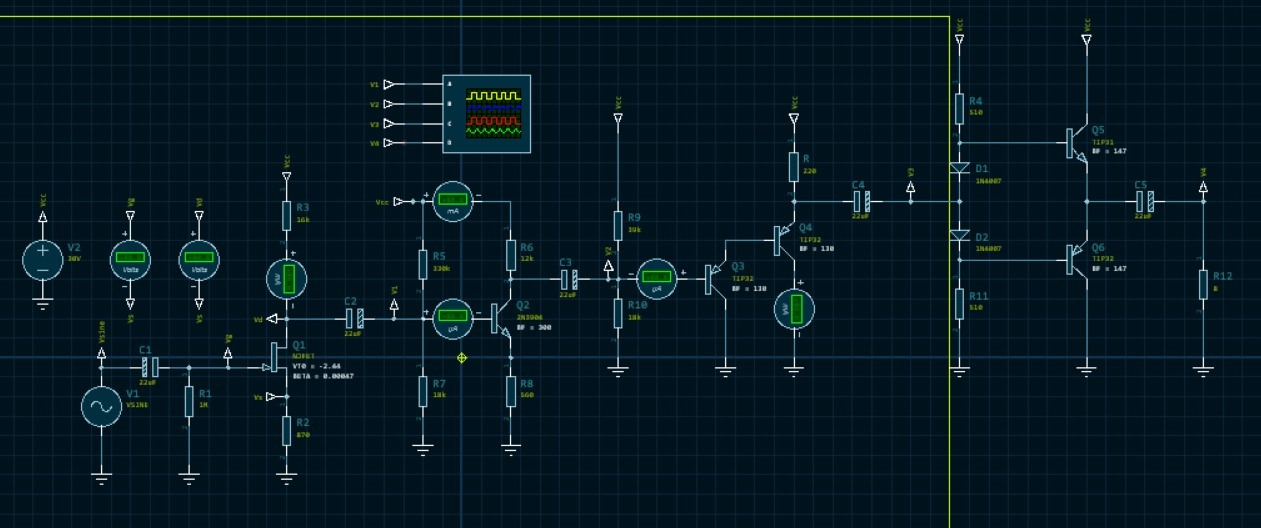
\includegraphics[width=0.9\textwidth]{img/fig09_proteus.jpg}
\caption{Diseño completo del amplificador multietapa en Proteus.}\label{fig:fig09_proteus}
\end{figure*}

\section{Resultados experimentales}
Las pruebas experimentales se realizaron inicialmente por etapas para verificar la coherencia entre los cálculos teóricos y las mediciones prácticas.

La Fig.~\ref{fig:fig10_senal_entrada} muestra la señal de audio del celular usada como entrada. Su valor RMS medido fue de 139.7 mV, con picos entre \(-297\) mV y \(+248\) mV, consistentes con la entrada de diseño de 200 mVp.

\begin{figure}[!htbp]\centering
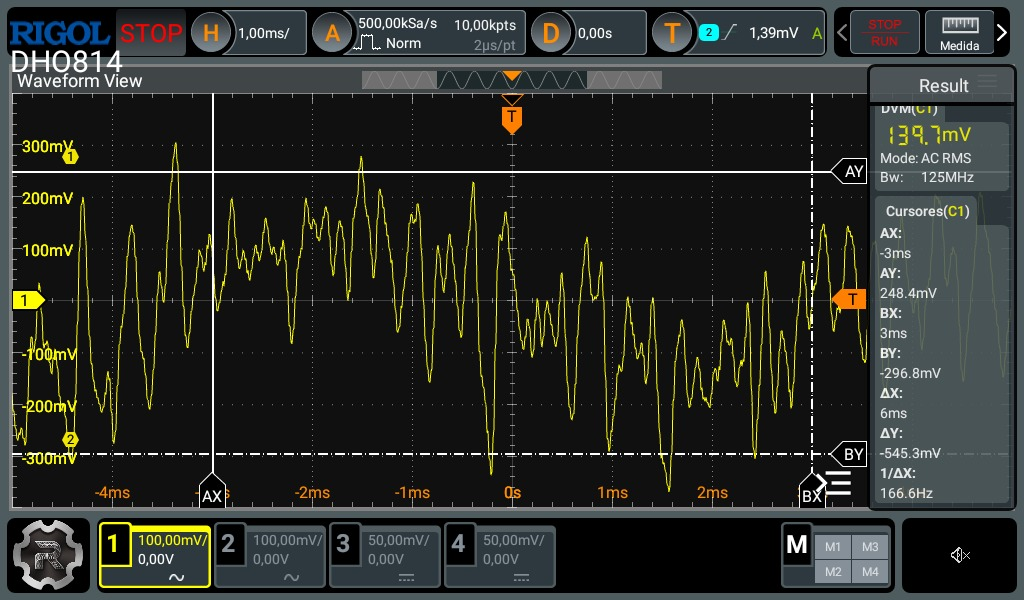
\includegraphics[width=0.95\columnwidth]{img/fig10_senal_entrada.jpg}
\caption{Señal de audio de entrada (celular): 139.7 mV RMS.}\label{fig:fig10_senal_entrada}
\end{figure}

Durante el montaje se presentaron problemas asociados a falsos contactos y daños en algunos pines de la protoboard, lo cual afectó inicialmente la transmisión de la señal (Figs.~\ref{fig:fig11_montaje_banco} y~\ref{fig:fig12_montaje_protoboard}). A pesar de estas dificultades, las pruebas individuales mostraron una correlación adecuada entre teoría y práctica. Posteriormente se integró el sistema completo, obteniendo funcionamiento correcto tanto en baja como en media potencia.

\fig{fig11_montaje_banco}{Banco de pruebas: fuentes, generador y osciloscopio.}{0.95}
\fig{fig12_montaje_protoboard}{Montaje experimental del amplificador multietapa en protoboard.}{0.85}

En las pruebas de baja potencia el sistema funcionó correctamente desde el primer intento. En media potencia fue necesario modificar algunas resistencias y reemplazar la protoboard debido a problemas técnicos del montaje.

La Fig.~\ref{fig:fig13_prueba_5khz} muestra una prueba con señal senoidal de 5 kHz: para una entrada de 101.1 mVpp se midió una salida de 3.03 Vpp, es decir, \(A_v \approx 30\) en el punto medido, sin distorsión visible.

\fig{fig13_prueba_5khz}{Prueba con senoidal de 5 kHz: entrada 101.1 mVpp (C1, amarillo) y salida 3.03 Vpp (C2, azul).}{0.95}

La Fig.~\ref{fig:fig14_salida_final} muestra la salida final con señal de audio. El canal 1 registró 18.0 Vpp con un máximo de 11.1 V. Con estos valores, la potencia instantánea pico sobre la carga fue
\begin{equation}
P_{pico} = \frac{(11.1\ \text{V})^2}{8\ \Omega} \approx 15.4\ \text{W},
\end{equation}
y la potencia promedio, estimada como la de una senoidal de igual amplitud, se encuentra entre
\begin{equation}
\frac{(9\ \text{V})^2}{2\cdot 8\ \Omega} \approx 5\ \text{W} \quad \text{y} \quad \frac{(11.1\ \text{V})^2}{2\cdot 8\ \Omega} \approx 7.7\ \text{W}.
\end{equation}
El sistema operó sin recalentamiento significativo en este rango, lo que indica que la etapa de potencia y la adaptación entre etapas fueron adecuadamente seleccionadas.

\fig{fig14_salida_final}{Salida final con señal de audio: 18.0 Vpp, \(V_{max} = 11.1\) V.}{0.9}

\subsection{Diseño PCB}
También se realizó el diseño PCB del sistema, mostrado en la Fig.~\ref{fig:fig15_pcb}; por limitaciones de tiempo no fue posible fabricar la baquela.

\fig{fig15_pcb}{Diseño PCB realizado en Proteus.}{0.95}

\section{Discusión}
El diseño evidenció la importancia de la adaptación de impedancias en sistemas multietapa. Se observó que pequeñas variaciones en la resistencia de entrada de una etapa modificaban considerablemente las condiciones de polarización de la anterior y la estabilidad global del circuito.

La utilización del Darlington permitió solucionar los problemas de baja ganancia de corriente y adaptación de impedancias, que no pudieron resolverse con una sola etapa CC.

Asimismo, se comprobó experimentalmente que la resistencia de carga de la etapa EC (\(\approx 12\) k\(\Omega\)) debía mantenerse menor que la de la etapa JFET (\(\approx 16\) k\(\Omega\)) para evitar valores excesivos de resistencia reflejada que afectaran el cálculo de \(R_B\).

Las pruebas prácticas también permitieron identificar limitaciones del uso de protoboard en sistemas de media potencia, especialmente falsos contactos y calentamiento localizado.

\section{Conclusiones}
Se diseñó e implementó un amplificador de potencia multietapa compuesto por una etapa JFET, una etapa emisor común, una etapa colector común Darlington y una etapa clase AB, capaz de amplificar la señal de audio de un celular hacia un parlante de \(8\,\Omega\).

El diseño teórico apunta a una ganancia total de voltaje de
\begin{equation}
A_v = A_{v(JFET)} \cdot A_{v(EC)} \approx 5 \cdot 10 = 50,
\end{equation}
ya que las etapas Darlington y clase AB tienen ganancia de voltaje cercana a la unidad y aportan principalmente ganancia de corriente.

Experimentalmente se alcanzaron picos de 11.1 V sobre la carga (\(\approx 15\) W instantáneos pico, entre 5 y 8 W promedio estimados), manteniendo estabilidad térmica.

La etapa JFET proporcionó alta impedancia de entrada, la etapa EC aportó la mayor parte de la ganancia de voltaje y la etapa Darlington resolvió la adaptación de impedancias hacia la etapa clase AB. Las observaciones experimentales fueron coherentes con los cálculos teóricos; sin embargo, la validación cuantitativa etapa por etapa no puede presentarse debido a la pérdida de los datos (Sección~\ref{sec:erratas}).

\section{Video de funcionamiento}
El funcionamiento completo del amplificador puede observarse en:
\url{https://www.youtube.com/watch?v=2Uj_PoNgtI4}

\section{Fe de erratas y nota sobre los datos}\label{sec:erratas}
Este documento es una versión corregida del informe entregado en el semestre 2026-1. Las mediciones originales tomadas durante las pruebas (puntos de operación DC y ganancias medidas por etapa) se perdieron después de la entrega. Por esta razón no se incluye una tabla comparativa entre valores teóricos y medidos, y los únicos datos cuantitativos experimentales son los que se pueden leer directamente en las capturas del osciloscopio (Figs.~\ref{fig:fig10_senal_entrada}, \ref{fig:fig13_prueba_5khz} y~\ref{fig:fig14_salida_final}).

Respecto a la versión original se corrigieron los siguientes errores:
\begin{enumerate}[leftmargin=1.4em]
\item \textbf{Potencia y unidades.} La versión original reportaba una potencia de 12~VA en el diseño y de 14 a 16~VA en las pruebas. El valor de diseño correspondía al producto \(V_p I_p = 10\ \text{V} \times 1.25\ \text{A}\), que es la potencia instantánea pico, no la potencia promedio; para una senoidal, la potencia promedio es la mitad (\(\approx 6.25\) W). El rango de 14--16 es consistente con la potencia instantánea pico para picos de 10.6--11.3 V, coherente con el máximo de 11.1 V medido en la Fig.~\ref{fig:fig14_salida_final}. Además, sobre una carga resistiva la unidad correcta es el vatio (W), no el voltamperio (VA).
\item \textbf{Transistores y beta del Darlington.} El texto original indicaba \(\beta \approx 1800\), mientras que las hojas de cálculo (Figs.~\ref{fig:fig07_calc_darlington_1} y~\ref{fig:fig08_calc_darlington_2}) usan \(h_{fe} = 18\,000\); este último es el valor correcto y es consistente con \(\beta_D \approx \beta^2\) para transistores de \(\beta \approx 134\). Además, la tabla de dispositivos indicaba dos TIP32C, pero la hoja de cálculo final está anotada como ``TIP 132''. Como los datos del montaje se perdieron, no es posible confirmar cuál de los dos dispositivos se usó finalmente.
\item \textbf{Tensión de alimentación.} Las Figs.~\ref{fig:fig05_calc_ec_1} y~\ref{fig:fig07_calc_darlington_1} usan \(V_{CC} = 30\) V, mientras que las Figs.~\ref{fig:fig01_calc_ab_1}, \ref{fig:fig06_calc_ec_2} y~\ref{fig:fig08_calc_darlington_2} usan 25 V. Las hojas de 30 V corresponden a una iteración preliminar; el diseño final opera con 25 V.
\item \textbf{Adaptación de impedancias.} El texto original afirmaba que el Darlington debía adaptarse a la etapa JFET y presentaba la diferencia entre 16 k\(\Omega\) y 12 k\(\Omega\) como un requisito no alcanzado. En realidad, 16 k\(\Omega\) es la resistencia de entrada de la etapa EC (carga del JFET) y 12 k\(\Omega\) es la resistencia de entrada del Darlington (carga de la etapa EC); ambos valores son consistentes con el diseño.
\item \textbf{Ganancia de corriente del Darlington.} El texto original reportaba \(A_i \approx 60\), valor de la primera iteración (Fig.~\ref{fig:fig07_calc_darlington_1}, \(A_i \approx 57\)). La iteración final (Fig.~\ref{fig:fig08_calc_darlington_2}) da \(A_i \approx 120\).
\item \textbf{Ganancia total de corriente.} Se aclaró que \(A_i = 6.25 \times 10^6\) supone una resistencia de entrada de 1 M\(\Omega\) en la etapa JFET.
\item \textbf{Signo de \(V_P\).} Para el JFET de canal N 2SK30, la tensión de estrangulamiento es negativa (\(V_P \approx -2.44\) V).
\item \textbf{Conclusiones.} Se reemplazó la afirmación de que el sistema alcanzó \(A_v \approx 50\) por la ganancia de diseño, ya que no se conserva una medición de la ganancia total. La única medición de ganancia disponible (Fig.~\ref{fig:fig13_prueba_5khz}) da \(A_v \approx 30\), pero no se registró en qué punto del circuito se tomó.
\item \textbf{Forma.} Se corrigió ``Universidad de ibagué'' y se ajustaron los títulos de las figuras para identificar la iteración de cálculo y la prueba que muestra cada una.
\end{enumerate}

\begin{thebibliography}{9}\footnotesize
\bibitem{sedra} A. Sedra y K. Smith, \emph{Microelectronic Circuits}, 7th ed. Oxford University Press, 2015.
\bibitem{boylestad} R. Boylestad y L. Nashelsky, \emph{Electronic Devices and Circuit Theory}, 11th ed. Pearson, 2013.
\bibitem{horowitz} P. Horowitz y W. Hill, \emph{The Art of Electronics}, 3rd ed. Cambridge University Press, 2015.
\bibitem{tip} Datasheet TIP31C/TIP32C, STMicroelectronics.
\bibitem{2n3904} Datasheet 2N3904, ON Semiconductor.
\bibitem{2sk30} Datasheet 2SK30 JFET.
\end{thebibliography}

\end{document}
